%%%%%%%%%%%%%%%%%%%%%%%%%%%%%%%%%%%%%%%%%%%%%%%%%%%%%%%%%%%%%%%
% IMPORTANTE: Cambiar el compilador a XeLaTeX en las opciones %
%          Plantilla ECI basada en U Pontificia Chile         %
%               Creditos Github: @diegocostares               %
%%%%%%%%%%%%%%%%%%%%%%%%%%%%%%%%%%%%%%%%%%%%%%%%%%%%%%%%%%%%%%%
\documentclass{style}
\addbibresource{bibliography/references.bib}

\begin{document}
	%%%%%%%%%%%%%%%%% RENOMBRE %%%%%%%%%%%%%%%%%
	\graphicspath{ {./img/} }
	\renewcommand{\contentsname}{Índice de contenido}
	\renewcommand{\listfigurename}{Índice de figuras}
	\renewcommand{\listtablename}{Índice de Tablas}
	\renewcommand{\tablename}{Tabla}
	\renewcommand{\figurename}{Imagen}
	\renewcommand*{\lstlistingname}{Código}
	
	
	%%%%%%%%%%%%%%%%% ENCABEZADO %%%%%%%%%%%%%%%%%
	% Si se quiere eliminar, se tiene que quitar tambien las configuraciones del style.cls
	\fancyhead[L]{ % Encabezado a la izquierda
		\begin{picture}(0,0) \put(0,30){
\includegraphics[width=25mm]{img/logo_eci.png}} \end{picture}
		\put(75,40){\textcolor{gray}{\scriptsize{\begin{tabular}{l}
						ESCUELA COLOMBIANA DE INGENIERÍA JULIO GARAVITO\\
						DEPARTAMENTO DE INGENIERÍA DE SISTEMAS
		\end{tabular}}}}
	}
	% Si se quiere agregar a la derecha remplazar:
	\rhead{} % Opcion 1
	%\rhead{\begin{picture}(0,0) \put(-85,12){\includegraphics[width=30mm]{img/IMAGEN.png}} \end{picture}} % Opcion 2
	
	
	%%%%%%%%%%%%%%%%% PORTADA %%%%%%%%%%%%%%%%%
	% Opcion 1: Importar un pdf tamaño carta de EEUU
	%\includepdf[pages=-]{img/Portada.pdf} % cambiar portada por pdf
	% Opcion 2: Escribir una portada completa
	\begin{titlepage}
	\begin{center}
		
		% Logo de la ECI
		\vspace*{-0.5cm}
		
\includegraphics[width=4.5cm]{img/logo_eci.png}
		
		\vspace{0.3cm}
		
		% Nombre completo de la universidad
		{\large \textbf{ESCUELA COLOMBIANA DE INGENIERÍA} \par}
		{\large \textbf{JULIO GARAVITO} \par}
		
		\vspace{0.3cm}
		

		
		% Título principal (MEDIFINDER)
		{\scshape\Huge \textbf{MediFinder} \par}
		
		\vspace{0.8cm}
		\rule{120mm}{0.8mm}
		\vspace{0.8cm}
		
		% Subtítulo
		{\Large \textbf{Búsqueda Inteligente de Medicamentos} \par}
		
		\vspace{1.5cm}
		
		% Descripción del proyecto
		{\normalsize Proyecto Final de la materia \par}
		{\normalsize Principios y Tecnologías de Inteligencia Artificial \par}
		
		\vspace{1.5cm}
		
		% Autores
		{\large \textbf{Autores:} \par}
		\vspace{0.3cm}
		{\normalsize 
			Mariana Malagón Tochoy \\[0.2cm]
			Ignacio Andrés Castillo Rendón \par}
		
		\vspace{1.2cm}
		
		% Profesor
		{\normalsize \textbf{Profesor:} Jossie Esteban Murcia Triviño \par}
		
		\vspace{1.5cm}
		
		% Universidad y facultad
		{\normalsize 
			Universidad Escuela Colombiana de Ingeniería Julio Garavito \\
			Facultad de Ingeniería de Sistemas \\[0.3cm]
			2026-1 \par}
		
		\vspace{0.5cm}
		
	\end{center}
\end{titlepage}
\newpage
	% Opcion 3: Sin portada - Se recomienda quitar indices
	
	%%%%%%%%%%%%%%%%% PRELIMINARES %%%%%%%%%%%%%%%%
	
	\section*{Declaración firmada}

\vspace{1cm}

"Declaro que he escrito este trabajo de investigación por mí mismo, y que no he utilizado otras fuentes o recursos que los indicados para su preparación. Declaro que he indicado claramente todas las citas directas e indirectas, y que este documento no se ha presentado en otro lugar para fines de examen o publicación"

\vspace{3cm}

\noindent\textbf{Nombre del estudiante \& Firma:}

\vspace{1.5cm}

\begin{center}
	\begin{tabular}{cc}
		% Firma de Mariana
		
\includegraphics[height=2cm]{img/firma_mariana.png} & 
		% Firma de Ignacio
		
\includegraphics[height=2cm]{img/firma_ignacio.png} \\[0.5cm]
		
		\rule{6cm}{0.4pt} & \rule{6cm}{0.4pt} \\
		Mariana Malagón Tochoy & Ignacio Andrés Castillo Rendón \\[0.3cm]
		Fecha: 17 de febrero de 2026 & Fecha: 17 de febrero de 2026 \\
	\end{tabular}
\end{center}

\pagebreak
	
	%%%%%%%%%%%%%%%%% INDICES %%%%%%%%%%%%%%%%%
	\setstretch{1}
	\tableofcontents
	\listoftables
	\listoffigures
	%\lstlistoflistings % Para hacer indice de codigo
	
	%%%%%%%%%%%%%%%%% ESPACIADO %%%%%%%%%%%%%%%%%
	\setstretch{1.15} 
	
	
	%%%%%%%%%%%%%%%%% CONTENIDO %%%%%%%%%%%%%%%%%
	\newpage
	%\input{content/tutorial} % HABILITAR Y DESHABILITAR PARA TENER EJEMPLOS
	\section*{Resumen}

Colombia enfrenta una crisis crítica en el sector salud derivada de la deuda acumulada de aproximadamente 32.9 billones de pesos entre 29 Entidades Promotoras de Salud (EPS), según informes del Ministerio de Salud emitidos en julio de 2025. Esta problemática financiera ha desencadenado graves consecuencias para las Instituciones Prestadoras de Servicios de Salud (IPS), generando desabastecimiento de medicamentos, demoras extensas en la entrega de fármacos y barreras de acceso para pacientes que dependen de tratamientos continuos. La Corte Constitucional ha constatado que persisten dificultades en la entrega de medicamentos por deudas acumuladas, incremento de tutelas y ausencia de información confiable para alertar sobre desabastecimientos.

Ante esta situación, el presente trabajo propone el desarrollo de un modelo de inteligencia artificial que brinde una solución temporal mientras se implementan reformas estructurales al sistema de salud. La propuesta consiste en un sistema integrado que combina Redes Neuronales Convolucionales (CNN) con el algoritmo K-Nearest Neighbors (KNN) para clasificar medicamentos a partir de imágenes y recomendar alternativas farmacéuticas similares. El modelo utiliza aprendizaje supervisado donde la CNN actúa como extractor de características, generando embeddings que permiten al KNN identificar medicamentos con componentes activos similares o presentaciones alternativas.

La solución implementa un pipeline de machine learning 100\% automatizado que, a partir de una fotografía del medicamento, clasifica su tipo (antibiótico, antiinflamatorio o analgésico), extrae información relevante del fármaco y recomienda alternativas disponibles basándose en similitud de componentes. Este enfoque busca empoderar a los pacientes con información oportuna mientras se resuelven los problemas estructurales del sistema de salud colombiano, mitigando el impacto de la crisis sobre personas con enfermedades crónicas o tratamientos de alto costo.

\subsection*{Palabras clave}
Medicamentos, EPS, IPS, Redes Neuronales, Algoritmo, Regresión, Clasificación, Modelo, Machine Learning

\section*{Abstract}

Colombia faces a critical crisis in the health sector derived from the accumulated debt of approximately 32.9 trillion pesos among 29 Health Promoting Entities (EPS), according to reports from the Ministry of Health issued in July 2025. This financial problem has triggered severe consequences for Health Service Provider Institutions (IPS), generating medicine shortages, extensive delays in drug delivery, and access barriers for patients who depend on continuous treatments. The Constitutional Court has confirmed that difficulties persist in medicine delivery due to accumulated debts, increased legal actions, and absence of reliable information to alert about shortages.

Facing this situation, the present work proposes the development of an artificial intelligence model that provides a temporary solution while structural reforms to the health system are implemented. The proposal consists of an integrated system that combines Convolutional Neural Networks (CNN) with the K-Nearest Neighbors (KNN) algorithm to classify medicines from images and recommend similar pharmaceutical alternatives. The model uses supervised learning where the CNN acts as a feature extractor, generating embeddings that allow the KNN to identify medicines with similar active components or alternative presentations.

The solution implements a 100\% automated machine learning pipeline that, from a photograph of the medicine, classifies its type (antibiotic, anti-inflammatory, or analgesic), extracts relevant information about the drug, and recommends available alternatives based on component similarity. This approach seeks to empower patients with timely information while structural problems of the Colombian health system are resolved, mitigating the crisis impact on people with chronic diseases or high-cost treatments.

\subsection*{Key words}
Medicines, EPS, IPS, Neural Networks, Algorithm, Regression, Classification, Modeling, Machine Learning

\pagebreak
	\section{Introducción}

\subsection{Problemas identificados}

Ante la crisis estructural del sistema de salud colombiano, se identificaron tres problemas principales que podrían beneficiarse de soluciones tecnológicas basadas en inteligencia artificial:

\subsubsection{Problema 1: Desabastecimiento de medicamentos y falta de alternativas}

Los pacientes enfrentan largas esperas y frecuentemente no encuentran los medicamentos prescritos en las farmacias. La falta de información sobre alternativas farmacéuticas con componentes activos similares genera frustración, abandono de tratamientos y deterioro de la salud, especialmente en personas con enfermedades crónicas.

\subsubsection{Problema 2: Ineficiencia en la gestión de inventarios farmacéuticos}

Las farmacias y gestores farmacéuticos carecen de sistemas predictivos que permitan anticipar desabastecimientos y optimizar la distribución de medicamentos. La falta de visibilidad en tiempo real sobre la disponibilidad de fármacos en diferentes puntos de la cadena de suministro genera pérdidas económicas y afecta la atención al paciente.

\subsubsection{Problema 3: Asimetría de información entre pacientes y el sistema de salud}

Los pacientes tienen acceso limitado a información confiable sobre sus medicamentos, alternativas disponibles, precios comparativos y disponibilidad en diferentes farmacias. Esta brecha informativa los deja en desventaja frente a un sistema de salud complejo y en crisis.

\subsection{Justificación como proyecto de Principios y Tecnologías de Inteligencia Artificial}

De los tres problemas identificados, se seleccionó el \textbf{Problema 1: Desabastecimiento de medicamentos y falta de alternativas} porque es ideal para un proyecto de PTIA por las siguientes razones:

\begin{itemize}
	\item \textbf{Requiere visión por computadora:} La identificación de medicamentos a partir de fotografías es un problema clásico de clasificación de imágenes que se beneficia de Redes Neuronales Convolucionales (CNN).
	
	\item \textbf{Involucra sistemas de recomendación:} Encontrar medicamentos similares basándose en componentes activos y características extraídas requiere algoritmos de aprendizaje automático como K-Nearest Neighbors (KNN).
	
	\item \textbf{Combina múltiples técnicas de IA:} El proyecto integra deep learning (CNN para clasificación) con machine learning tradicional (KNN para recomendación), permitiendo explorar diferentes enfoques y compararlos.
	
	\item \textbf{Permite aprendizaje supervisado:} Se puede entrenar el modelo con un dataset etiquetado de medicamentos, aplicando técnicas de data augmentation, transfer learning y fine-tuning.
	
	\item \textbf{Tiene métricas evaluables:} Es posible medir el desempeño del sistema con métricas estándar como accuracy, precision, recall y F1-score para clasificación, y métricas de similitud para recomendación.
	
	\item \textbf{Escalabilidad y mejora continua:} El modelo puede mejorarse continuamente con más datos, explorando arquitecturas más avanzadas como ResNet, EfficientNet o Vision Transformers.
\end{itemize}

\subsection{Contexto de la crisis del sistema de salud colombiano}

En los últimos años se ha venido presentando una problemática país con respecto al sector de salud, específicamente hacia el sector de las EPS (Entidad Promotora de Salud), en donde hace dos años el presidente vigente Gustavo Petro denunció reportes fraudulentos sobre la distribución de sus recursos para la atención en salud y fue el año pasado que, según informes presentados por el Ministerio de Salud el 15 de Julio del 2025, comenta que esa deuda (en el cual reúne al menos 29 EPS) es de aproximadamente 35 billones de dólares \cite{minsalud2025}. Esta deuda genera una crisis en el sistema de salud porque el gobierno está acorralando y asfixiando a una posible liquidez de las IPS (Instituciones Prestadoras de Servicios de Salud), provocando el cierre de servicios, falta de pagos a médicos, desabastecimiento de medicamentos y barreras de acceso para pacientes. La problemática financiera desencadena una serie de conflictos, no solamente en la sostenibilidad de hospitales y clínicas, como demoras y falta de medicamentos.

Bajo esta naciente preocupación, donde aumenta de sobremanera los tiempos de espera para su distribución, afectando la continuidad de los tratamientos, en el último año se han venido haciendo cada vez más evidentes. Acorde a una investigación por parte de la Corte Institucional, nos demuestra la realidad, la cual no es nada favorable:

\begin{quote}
	``La Corte Constitucional constató que persisten graves dificultades en la entrega de fármacos por deudas acumuladas entre EPS y gestores farmacéuticos, incremento de tutelas de pacientes, retrasos en trámites del Invima y ausencia de información confiable para alertar los desabastecimientos.'' \cite{colprensa2025}
\end{quote}

Se han ido proponiendo e implementando estrategias desde que inició el año para mitigar los daños, aparte de los ya presentes, entre ellas que el estado se haga cargo de los recursos de las EPS y que estas ultimas se encarguen solamente de prestar un servicio únicamente de gestores de vida y salud, además de un fuerte aumento en el presupuesto de los recursos destinados al sector salud.

Sin embargo, toda esta problemática sobre el asunto de los medicamentos no es algo que podrá encontrar una solución de manera inmediata porque a pesar de que estalló con la deuda de las EPS, es algo que venía de años atrás. Aún así, la sociedad colombiana no se puede quedar esperando por una respuesta positiva por parte de las entidades de salud tanto tiempo, porque la brecha que irá dejando a su paso será inmensa.

No es un tema sencillo de resolver, pero en unión con las innovaciones y revoluciones utilizando la tecnología como medio, se puede encontrar aquel punto óptimo, así mientras se termina de dar el camino más adecuado para el sector salud en Colombia, la sociedad colombiana no termine siendo los más afectados ante todo este conflicto.

\pagebreak
	\section{Trabajos Relacionados}

Esta sección presenta una revisión de trabajos previos relacionados con la clasificación de medicamentos mediante inteligencia artificial y sistemas de recomendación farmacéuticos.

\subsection{Clasificación de medicamentos mediante visión por computadora}

\subsubsection{Trabajo 1: Drug Identification System usando CNN}

Kumar et al. (2019) desarrollaron un sistema de identificación de medicamentos mediante deep learning que utiliza CNN para clasificar píldoras y tabletas a partir de imágenes.

\textbf{Tecnología utilizada:}
\begin{itemize}
	\item Red Neuronal Convolucional (CNN) con 6 capas convolucionales
	\item Transfer learning con ImageNet
	\item Framework: TensorFlow y Keras
\end{itemize}

\textbf{Resultados:}
\begin{itemize}
	\item Accuracy: 94.3\%
	\item Tiempo de inferencia: 0.8 segundos por imagen
\end{itemize}

\subsubsection{Trabajo 2: Pill Recognition usando ResNet-50}

Zeng et al. (2020) utilizaron ResNet-50 con fine-tuning específico para reconocimiento de medicamentos.

\textbf{Tecnología utilizada:}
\begin{itemize}
	\item ResNet-50 pre-entrenada
	\item Data augmentation avanzado
	\item Framework: PyTorch
\end{itemize}

\textbf{Resultados:}
\begin{itemize}
	\item Accuracy: 96.7\%
	\item Top-5 accuracy: 99.1\%
\end{itemize}

\subsection{Sistemas de recomendación farmacéuticos}

\subsubsection{Trabajo 3: Drug Recommendation usando Sentiment Analysis}

Doshi et al. (2021) propusieron un sistema de recomendación basado en análisis de sentimientos y componentes activos.

\textbf{Tecnología utilizada:}
\begin{itemize}
	\item Natural Language Processing (NLP)
	\item K-Nearest Neighbors para medicamentos similares
	\item Filtrado colaborativo
\end{itemize}

\textbf{Resultados:}
\begin{itemize}
	\item Precisión en recomendaciones: 87.5\%
	\item Satisfacción de usuarios: 78\%
\end{itemize}

\subsubsection{Trabajo 4: Content-Based Drug Recommendation}

Park et al. (2022) desarrollaron un sistema basado en similitud de componentes activos usando autoencoders.

\textbf{Tecnología utilizada:}
\begin{itemize}
	\item Autoencoder para embeddings de medicamentos
	\item Similitud coseno en espacio latente
	\item Base de datos FDA
\end{itemize}

\textbf{Resultados:}
\begin{itemize}
	\item Precisión: 91.2\%
	\item Recall: 85.7\%
\end{itemize}

\subsection{Diferenciación del proyecto MediFinder}

MediFinder integra ambas líneas de investigación:

\begin{itemize}
	\item Pipeline completo: desde captura de imagen hasta recomendación
	\item CNN para clasificación + KNN para recomendación
	\item Contextualizado a Colombia
\end{itemize}

\pagebreak    % ← LÍNEA NUEVA AGREGADA
	\section{Descripción y caracterización detallada del problema}

\subsection{Criterios de selección del problema}

De los tres problemas identificados en la Introducción, se seleccionó el desabastecimiento de medicamentos y falta de alternativas usando los siguientes criterios:

\begin{enumerate}
	\item \textbf{Impacto social medible:} Afecta directamente a pacientes con enfermedades crónicas. En 2024 se registraron más de 150,000 tutelas relacionadas con falta de acceso a medicamentos.
	
	\item \textbf{Urgencia temporal:} Crisis activa que requiere soluciones inmediatas.
	
	\item \textbf{Viabilidad técnica con IA:} Puede abordarse con CNN y KNN existentes.
	
	\item \textbf{Disponibilidad de datos:} Existen fuentes públicas (INVIMA, MinSalud).
	
	\item \textbf{Factibilidad de implementación:} Solución de software más rápida que cambios estructurales.
	
	\item \textbf{Empoderamiento del usuario:} Pone información directamente en manos de pacientes.
	
	\item \textbf{Escalabilidad:} Puede expandirse fácilmente a más medicamentos y usuarios.
\end{enumerate}

\subsection{Caracterización detallada del problema seleccionado}

La Universidad Javeriana en un estudio, comenta que el asunto no reside en la ausencia física de los medicamentos, sino que, tal y como mencionaba el Universal, es en todo el abastecimiento, precisamente por toda la crisis financiera que vienen arrastrando \cite{diaz2025}.

La falta de abastecimiento y entrega de medicamentos no solo afecta a los pacientes sino también a hospitales. Durante el año pasado, por suspensión de actividades de empresas que se encargaban de la producción de medicamentos a nivel nacional, el Ministerio de Salud emitió que llegó a haber una escasez de fármacos vitales, tales como la norepinefrina o la vasopresina (usados en UCI principalmente). A saber: En el caso de la norepinefrina, el mercado está cubierto en un 26\% por Laboratorios Ryan, que dispone de 120.000 ampollas mensuales entre septiembre y diciembre. Sin embargo, esta cantidad no ha sido suficiente para cubrir la demanda, motivo por el cual el medicamento permanece en la lista de vital no disponible desde 2018.

Debido a esto, se tuvieron que otorgar licencias y autorizaciones de importación a empresas externas para un correcto abastecimiento, en donde gracias a las empresas como Holland Group, Pisa Farmacéutica, Reprefarco y Sicmafarma, pudieron llegar de la mano de Reprefarco unas 100.000 unidades, además de la empresa Nextpharmasourcing que otorgó 3.700 cajas de 10 ampollas cada una, dando un gasto más a todo el que se viene arrastrando \cite{saavedra2025}.

Asimismo, a pesar de que se viene incrementando el desembolso por parte de los colombianos en la compra de medicamentos, dando un crecimiento en el gasto privado, no garantiza una traducción en acceso oportuno a estos medicamentos, en donde se presentan demoras extensas, además de una falta de disponibilidad y un alza en los precios, generando una presente y creciente sensación de inconformismo entre la sociedad dependientes de los medicamentos (enfermedades crónicas, patologías huérfanas o tratamientos de alto costo como el cáncer) \cite{calero2025}.

% PRIMERA IMAGEN - Tabla de categorías del gasto
\begin{figure}[H]
	\centering
	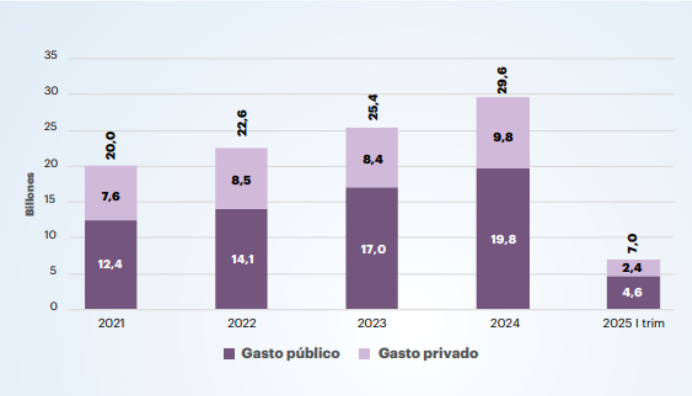
\includegraphics[width=0.90\textwidth]{img/gasto.png}
	\caption{Detalle del gasto en salud por categorías 2021-2025}
	\label{fig:gasto}
\end{figure}

% SEGUNDA IMAGEN - Gráfica de evolución
\begin{figure}[H]
	\centering
	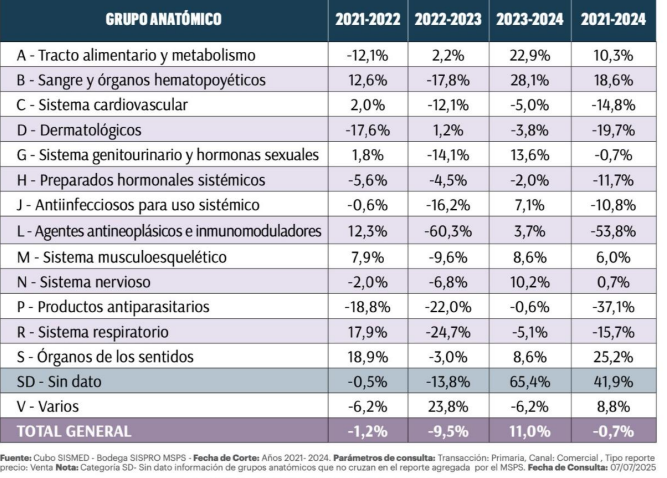
\includegraphics[width=0.85\textwidth]{img/evolucionGasto.png}
	\caption{Evolución del gasto privado en medicamentos en Colombia 2021-2025}
	\label{fig:evolucion}
\end{figure}

Como se puede evidenciar en las gráficas anteriores, el gasto privado en salud se fue en alza en los últimos años, pasando de ser de 20 billones a 29.2 billones entre 2021 y 2024, además de un aumento nominal del 48.0\% y del 13.8\% después de inflación.

Igualmente es válido mencionar que el gasto en medicamentos no incluye los costos adicionales asociados a la gestión para la disposición de las medicinas en los gestores farmacéuticos o prestadores de servicios de salud \cite{acemi2025}.

Como bien se mencionó previamente, no es un tema sencillo de encontrarle y/o darle una solución exacta, para la magnitud que representa ante una sociedad donde existe un grupo de personas que dependen de medicamentos para su día a día debido a distintas complicaciones. Del mismo modo, al ser una situación país grande, se genera la falsa esperanza que será el gobierno que logre solucionar todo en tiempo récord y la sociedad se quedará esperando hasta que exista una garantía, pero esa espera solo genera una cadena dominó de más problemas, en vez de poder darle alternativas y soluciones temporales utilizando la tecnología como medio para ello.

\pagebreak
	\section{Objetivos}

\subsection{Objetivo general}
Estudiar la situación país sobre las problemáticas de la deuda de las EPS y todos sus desencadenantes; ante ello, colocar el foco sobre el tema de los medicamentos y buscar la solución adecuada de un modelo de inteligencia artificial que otorgue un apoyo a todo este conflicto crítico.

\subsection{Objetivos específicos}
\begin{enumerate}
	\item Investigar alternativas ya implementadas sobre programas y/o modelos IA que ayuden al paciente a la búsqueda de alternativas para un medicamento y le informe al paciente sobre el medicamento.
	
	\item Hacer una investigación de IA en la búsqueda de alternativas para un medicamento mediante KNN.
	
	\item Hacer una investigación de IA en la búsqueda de alternativas para clasificación de medicamentos mediante CNN.
	
	\item Realizar un prototipo (MVP) del modelo IA planteado.
\end{enumerate}

\pagebreak
	\section{Marco Teórico}

\subsection{EPS e IPS}

Puede llegar a existir la confusión entre estos dos términos los cuales provienen de la Ley 100 la cual reglamenta el sistema de salud colombiano y provee las herramientas para la financiación y sostenibilidad de su estructura procurando garantizar una atención igualitaria para todas las personas.

En primer lugar, las EPS, Entidades Promotoras de Salud, son las responsables de la afiliación y el registro de los afiliados y del recaudo de sus cotizaciones. Como dice artículo publicado por la Alcaldía de Bogotá:

\begin{quote}
	Su función básica es organizar y garantizar la prestación del Plan Obligatorio de Salud (POS) y hacer los giros respectivos al Fondo de Solidaridad y Garantía que es donde se administran los recursos del Sistema de Seguridad Social en Salud. Así, todas las personas se afilian a estas y quedan amparados en su intermediación para acceder a los servicios médicos. \cite{arias2021}
\end{quote}

Por otro lado, las IPS, Instituciones Prestadoras de Servicios de Salud, corresponden a todas las entidades, asociaciones y/o personas bien sean públicas, privadas o con economía mixta, que están autorizadas para prestar de forma parcial y/o total los procedimientos que se demanden para cumplir el Plan Obligatorio de Salud (POS). Dentro de este grupo es que entran los hospitales, clínicas y distintos centros de salud.

\subsection{Deuda de las EPS}

El año pasado, mediante un boletín de prensa, el número 093-2025, del día 15 de Julio, emitió el último informe (hasta ese momento) por parte de la Contraloría General de la República sobre la situación financiera del sistema de salud que revela 29 Entidades Promotoras de Salud (EPS) acumulan una deuda que asciende a los \$32,9 billones de pesos por servicios prestados por clínicas, hospitales, laboratorios, operadores farmacéuticos y otros actores del sistema.

Esta cifra, como bien se da en el informe dado por la Contraloría, representó un aumento de \$7.9 billones comparado al monto reportado en 2023, lo cual claramente refleja un desorden a nivel económico desde la parte administrativa en el que se encuentra todo el sistema de salud, que como expresan en el reporte, es ``debido al actual modelo de aseguramiento basado en la intermediación.'' \cite{minsalud2025}

Como consecuencia a ello, la deuda en primera instancia afecta gravemente la estabilidad de los prestadores y proveedores de servicios, pero se genera una cadena llegando a afectar también de sobremanera a los usuarios, en donde se llega a violar el derecho fundamental a la salud en escenarios como barrera en el acceso con los largos retrasos para citas y cirugías, el desabastecimiento de insumos médicos y tecnologías necesarias y llegando a declararlo ya como emergencia humanitaria (por parte de AFIDRO - Asociación de Laboratorios Farmacéuticos de Investigación).

Es válido mencionar que, dentro de este boletín, lo dicho es que la culpa no recae en el gobierno, sino que va directamente a las EPS, de sus decisiones, omisiones y su mala organización administrativa.

\subsection{Redes Neuronales Convolucionales (CNN)}

Para poder definir las redes neuronales convolucionales, en primer lugar, toca dar paso a la definición y el funcionamiento de las redes neuronales en sí.

IBM, dentro de su página web, brinda la definición al respecto de este tema:

\begin{quote}
	Las redes neuronales son un subconjunto del machine learning y están en el corazón de los algoritmos de deep learning. Están compuestas por capas de nodos, que incluyen una capa de entrada, una o más capas ocultas y una capa de output. Cada nodo está conectado a otro y tiene un peso y un umbral asociados. \cite{ibm2025cnn}
\end{quote}

Es válido hacer la mención de la definición general de las redes neuronales debido a que existen varios tipos usados para distintos casos y para distintos tipos de datos. Por ejemplo, las redes neuronales recurrentes se suelen usar para el procesamiento del lenguaje natural y el reconocimiento de voz. Y están las redes neuronales convolucionales, que son utilizadas principalmente para tareas de clasificación y computer vision.

El funcionamiento de este tipo de redes neuronales es destacable en el área de imágenes, voz o audio, y se componen de tres tipos de capas (principalmente): capa convolucional, capa de agrupación y la capa totalmente conectada.

La capa convolucional es la primera capa de una red convolucional. Si bien las capas convolucionales pueden ir seguidas de otras capas convolucionales o de capas de agrupación, la capa final es la capa totalmente conectada. Con cada capa, la CNN aumenta su complejidad, identificando mayores porciones de la imagen. Las primeras capas se centran en características simples, como colores y bordes. A medida que los datos de la imagen avanzan a través de las capas, la CNN comienza a reconocer elementos o formas más grandes hasta que finalmente identifica el objeto esperado.

\subsection{K-Nearest Neighbors (KNN)}

Por otro lado, la IA que se adaptará ante la problemática descrita no solo se basará en una clasificación utilizando la CNN, sino que una parte del modelo utilizará este algoritmo, usado actualmente para Machine Learning.

En su definición, el algoritmo de k-nearest neighbors (KNN) es un clasificador de aprendizaje supervisado no paramétrico, que emplea la proximidad para realizar clasificaciones o predicciones sobre la agrupación de un punto de datos individual. Hoy en día, es uno de los clasificadores de clasificación y regresión más sonados además de sencillos de implementar.

El uso principal del algoritmo KNN es de clasificación, en donde se basa o parte del supuesto de que se pueden encontrar puntos similares cercanos uno del otro. Tipo como si fuera un grafo, los dos hijos del padre.

Ante la explicación precisa del funcionamiento del supuesto de que hay puntos similares cercanos, dentro de la página de IBM:

\begin{quote}
	En los problemas de clasificación, la etiqueta de clase se asigna por mayoría de votos, es decir, se emplea la etiqueta que se representa con más frecuencia en torno a un punto de datos determinado. Aunque técnicamente se considera ``votación por pluralidad'', el término ``votación por mayoría'' se emplea más comúnmente en las publicaciones al respecto. La distinción entre estas terminologías es que la ``votación por mayoría'' requiere técnicamente una mayoría superior al 50\%, lo que funciona sobre todo cuando sólo hay dos categorías. Cuando hay varias clases, por ejemplo, cuatro categorías, usted no requiere necesariamente el 50\% de los votos para llegar a una conclusión sobre una clase, ya que podría asignar una etiqueta de clase con un voto superior al 25\%. \cite{ibm2025knn}
\end{quote}

\pagebreak
	\section{Propuesta de solución}

Reuniendo todo lo mencionado ante la problemática presente en la sociedad colombiana, que de paso no será algo que se solucione en el corto plazo y el país necesita una solución al menos temporal mientras todo retoma su ``curso normal''.

La solución planteada es implementar un modelo IA que tenga un aprendizaje automatizado supervisado (CNN) y no supervisado (KNN), el cual se entrenará previamente con la mayor cantidad de datos que logremos conseguir, en donde el paciente sube la foto de un medicamento, bajo un contexto que fue un medicamento que utilizó previamente más ahora que lo volvió a buscar se dio cuenta que ya se le acabó, entonces, el modelo se encargará de darle al paciente/persona información sobre ese medicamento (su tipo, si es analgésico, antibiótico o antiinflamatorio, y de paso información como tal del medicamento). De igual manera, se le dará al paciente recomendaciones del fármaco que colocó, sea que tenga el mismo componente a que tenga un componente parecido, pero que, de todas formas, le funcione a la persona para que lo pueda conseguir en caso de que el que tenía que se le agotó, se le complique conseguirlo.

\subsection{Arquitectura del sistema}

Mediante el conocimiento que tenemos sobre implementar modelos IA en código, inicialmente vamos a empezar a implementar todo con las librerías Scikit-learn + TensorFlow/PyTorch en Python, para no tener que definir todo desde cero. Igualmente, en caso de que sea necesario implementarlo desde cero, se hará definiendo todas las funciones básicas para que el modelo funcione de manera correcta.

Tener en cuenta que toca tener metadata asociada, pero toda la búsqueda de similitud es trabajo 100\% de ML, en donde:

\subsubsection{Durante entrenamiento}

\begin{itemize}
	\item Guardas los embeddings de todos los medicamentos del training set
	\item Guardas metadata asociada (nombre, componente, usos)
\end{itemize}

\subsubsection{Durante inferencia}

\begin{itemize}
	\item CNN extrae embedding del medicamento nuevo
	\item KNN busca en el espacio de embeddings (no en una BD tradicional)
	\item KNN retorna los K vecinos + su metadata
\end{itemize}

La clave está en que el KNN trabaja en el espacio latente aprendido por la CNN, no en una base de datos relacional.

\pagebreak
	\section{Análisis de resultados}

\textit{Todavía no hecho - Esta sección se completará una vez se obtengan los resultados experimentales del modelo implementado.}

\pagebreak
	\section{Conclusiones}

Se estima que, mediante esta implementación del modelo IA entrenado para dar medicamentos similares, se logre brindar una solución temporal ante la problemática de la deuda y sus desencadenantes, pero también lograr implementarla de mejor manera como una ayuda a las personas, unido con entidades del sector de la salud, para brindar ese apoyo ante recomendaciones de fármacos aptos para cada situación que pueda estar viviendo cada paciente.

\pagebreak
	
	
	%%%%%%%%%%%%%%%%% BIBLIOGRAFIA %%%%%%%%%%%%%%%%%
	\newpage
	\printbibliography
	
	%%%%%%%%%%%%%%%%%%% ANEXOS %%%%%%%%%%%%%%%%%%%%%
	
	\newpage
	%\input{anexos/anexo_LaTeX} % HABILITAR Y DESHABILITAR PARA TENER EJEMPLOS
	
\end{document}